% Ch4: overall VAE-DiT architecture (inference path, with the training target noted).
% Shapes: 4 channels x 101 frames x 256^2 -> pad to 105 -> LTX VAE (8x temporal,
% 32x spatial, 128 latent channels) -> z in R^{128 x 14 x 8 x 8}.
% gamma -> Fourier features (64) -> MLP (256) -> 4 tokens of width 4096 -> DiT cross-attention.
% First-frame conditioning: the latent frame z_0 of the initial condition stays clean,
% the DiT denoises z_{1:13}. Decoder output is cropped back to 101 frames.
\documentclass[tikz,border=4pt]{standalone}
\usepackage{amsmath,amssymb}
\usetikzlibrary{arrows.meta,positioning,calc,fit,backgrounds}
% Shared colours for the thesis TikZ figures. Same reference palette as
% scripts/thesis_figures.py (dataviz light mode), so diagrams and plots match.
\definecolor{ink}{HTML}{0B0B0B}
\definecolor{ink2}{HTML}{52514E}
\definecolor{muted}{HTML}{898781}
\definecolor{hair}{HTML}{C3C2B7}
\definecolor{neutralfill}{HTML}{F0EFEC}
\definecolor{blue}{HTML}{2A78D6}
\definecolor{bluefill}{HTML}{CDE2FB}
\definecolor{bluedark}{HTML}{184F95}
\definecolor{orange}{HTML}{EB6834}
\definecolor{orangefill}{HTML}{FBE0D3}
\definecolor{aqua}{HTML}{1BAF7A}
\definecolor{aquafill}{HTML}{D2F0E4}
\definecolor{violet}{HTML}{4A3AA7}
\definecolor{violetfill}{HTML}{E3E0F6}

% Trainable modules: orange fill + solid border. Frozen: neutral fill,
% dashed border, and every figure also labels the state in text.
\tikzset{
  every node/.style={font=\small, text=ink},
  box/.style={draw=hair, rounded corners=2pt, align=center, inner sep=4pt, line width=0.6pt},
  trainable/.style={box, fill=orangefill, draw=orange, line width=0.8pt},
  frozen/.style={box, fill=neutralfill, draw=muted, dashed},
  data/.style={box, fill=bluefill, draw=blue},
  latent/.style={box, fill=violetfill, draw=violet},
  cond/.style={box, fill=aquafill, draw=aqua},
  arr/.style={-{Stealth[length=5pt]}, draw=ink2, line width=0.7pt},
  note/.style={font=\footnotesize, text=ink2, align=center},
}


\begin{document}
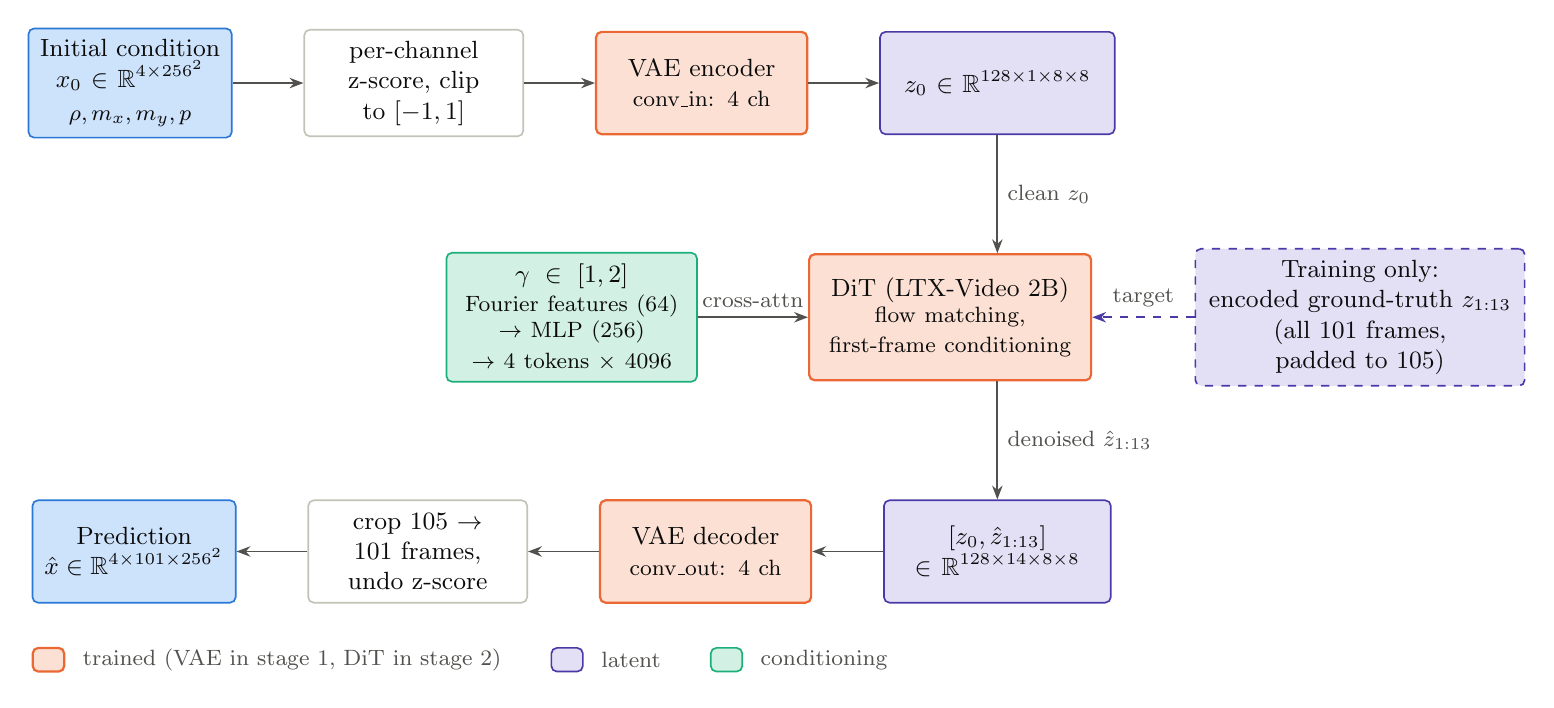
\begin{tikzpicture}[node distance=0.9cm]
  % ---- top row: encode --------------------------------------------------
  \node[data, minimum height=1.3cm, text width=2.3cm] (x) {Initial condition\\$x_0 \in \mathbb{R}^{4\times 256^2}$\\[1pt]\footnotesize$\rho, m_x, m_y, p$};
  \node[box, right=of x, minimum height=1.3cm, text width=2.5cm] (prep) {per-channel\\z-score, clip to $[-1,1]$};
  \node[trainable, right=of prep, minimum height=1.3cm, text width=2.4cm] (enc) {VAE encoder\\\footnotesize conv\_in: 4 ch};
  \node[latent, right=of enc, minimum height=1.3cm, text width=2.7cm] (z0) {$z_0 \in \mathbb{R}^{128\times 1\times 8\times 8}$};

  % ---- middle: DiT --------------------------------------------------------
  \node[trainable, below=1.5cm of z0, minimum height=1.6cm, text width=3.3cm, xshift=-0.6cm] (dit)
    {DiT (LTX-Video 2B)\\\footnotesize flow matching,\\ first-frame conditioning};
  \node[cond, left=1.4cm of dit, text width=2.9cm, minimum height=1.6cm] (emb)
    {$\gamma \in [1,2]$\\[1pt]\footnotesize Fourier features (64)\\ $\to$ MLP (256)\\ $\to$ 4 tokens $\times$ 4096};

  % ---- bottom row: decode -------------------------------------------------
  \node[latent, below=1.5cm of dit, text width=2.6cm, minimum height=1.3cm, xshift=0.6cm] (zhat)
    {$[z_0, \hat z_{1:13}]$\\$\in \mathbb{R}^{128\times 14\times 8\times 8}$};
  \node[trainable, left=of zhat, minimum height=1.3cm, text width=2.4cm] (dec) {VAE decoder\\\footnotesize conv\_out: 4 ch};
  \node[box, left=of dec, minimum height=1.3cm, text width=2.5cm] (post) {crop 105 $\to$ 101 frames,\\undo z-score};
  \node[data, left=of post, minimum height=1.3cm, text width=2.3cm] (xhat) {Prediction\\$\hat x \in \mathbb{R}^{4\times 101\times 256^2}$};

  \draw[arr] (x) -- (prep);
  \draw[arr] (prep) -- (enc);
  \draw[arr] (enc) -- (z0);
  \draw[arr] (z0.south) -- node[right, note] {clean $z_0$} (z0.south |- dit.north);
  \draw[arr] (emb) -- node[above, note] {cross-attn} (dit);
  \draw[arr] (dit.south -| zhat.north) -- node[right, note] {denoised $\hat z_{1:13}$} (zhat.north);
  \draw[arr] (zhat) -- (dec);
  \draw[arr] (dec) -- (post);
  \draw[arr] (post) -- (xhat);

  % training target, drawn to the right
  \node[latent, right=1.3cm of dit, text width=3.9cm, dashed, minimum height=1.6cm] (tgt)
    {Training only:\\encoded ground-truth $z_{1:13}$\\(all 101 frames, padded to 105)};
  \draw[arr, dashed, draw=violet] (tgt) -- node[above, note] {target} (dit);

  % legend
  \node[trainable, minimum width=0.4cm, minimum height=0.3cm, inner sep=0pt, below=0.55cm of xhat.south west, anchor=north west] (l1) {};
  \node[note, right=0.1cm of l1, anchor=west] (l1t) {trained (VAE in stage 1, DiT in stage 2)};
  \node[latent, minimum width=0.4cm, minimum height=0.3cm, inner sep=0pt, right=0.5cm of l1t] (l2) {};
  \node[note, right=0.1cm of l2, anchor=west] (l2t) {latent};
  \node[cond, minimum width=0.4cm, minimum height=0.3cm, inner sep=0pt, right=0.5cm of l2t] (l3) {};
  \node[note, right=0.1cm of l3, anchor=west] {conditioning};
\end{tikzpicture}
\end{document}
